%%%%%%%%%%%%%%%%%%%%%%%%%%%%%%%%%%%%%%%%%
% Szablon pracy dyplomowej
% Wydział Informatyki 
% Zachodniopomorski Uniwersytet Technologiczny w Szczecinie
% autor Joanna Kołodziejczyk (jkolodziejczyk@zut.edu.pl)
% Bardzo wczesnym pierwowzorem szablonu był
% The Legrand Orange Book
% Version 5.0 (29/05/2025)
%
% Modifications to LOB assigned by %JK
%%%%%%%%%%%%%%%%%%%%%%%%%%%%%%%%%%%%%%%%%

%----------------------------------------------------------------------------------------
%	CHAPTER 0
% 	author: Patryk Rakowski (rp51626@zut.edu.pl)
%----------------------------------------------------------------------------------------

\chapter{Analiza istniejących rozwiązań}
\label{rozdzial0}

W ramach analizy rynku zostały zostały przeanalizowane istniejące dotychczas rozwiązania służące do dokumentowania i analizy obserwacji ptaków. 
Obserwacje i wnioski zostały opisane poniżej.

\section{Ornitho.pl}

\begin{figure}[!htb]
	\centering
	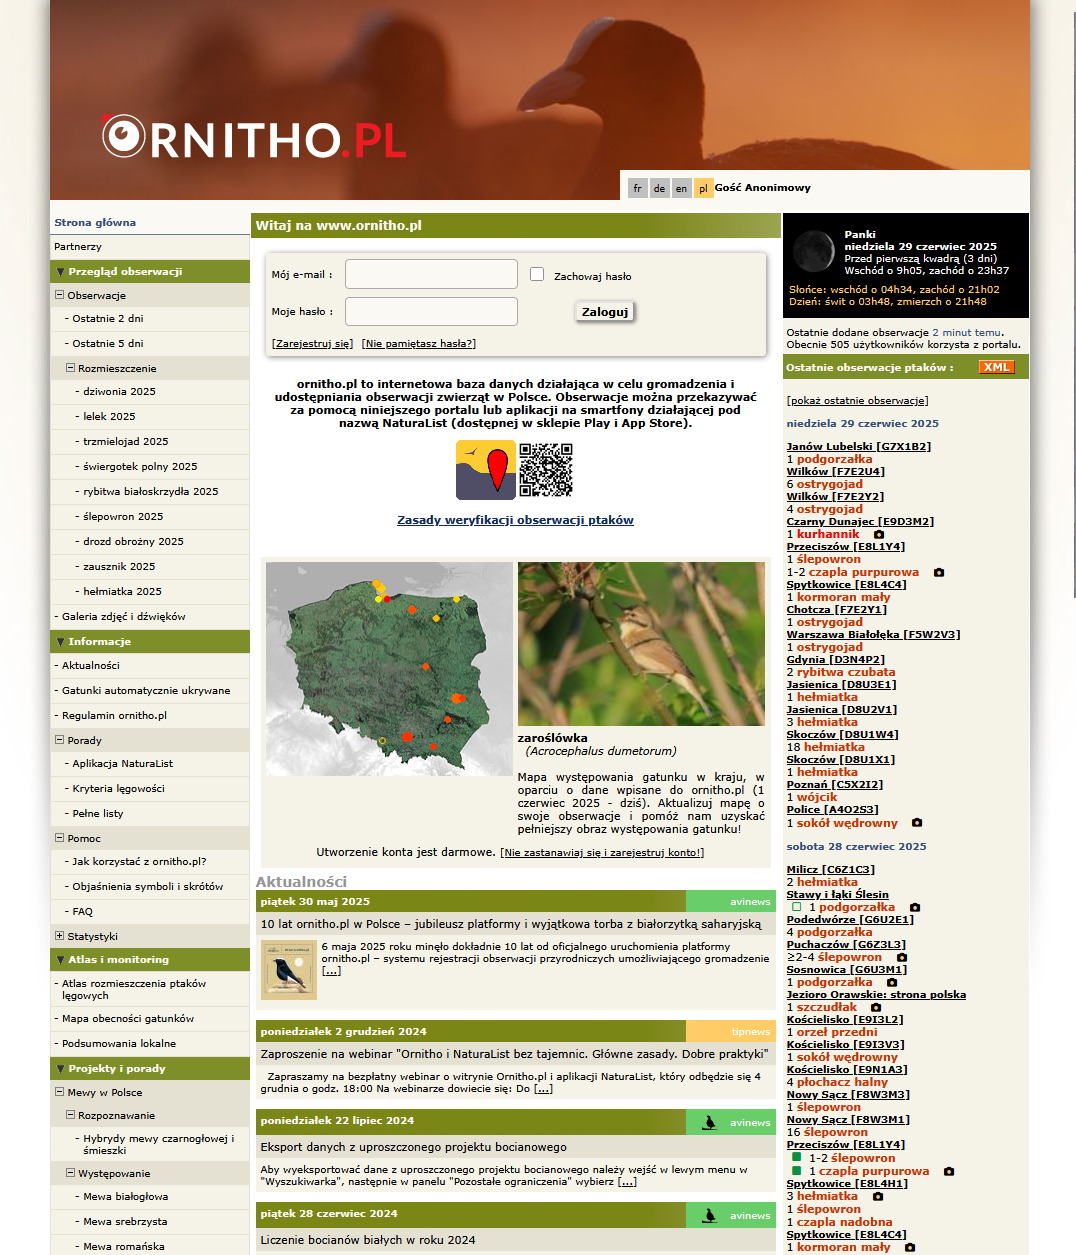
\includegraphics[width=0.6\textwidth]{/chapter0/ornithopl.png}
	\caption{Strona Ornitho.pl}
	\label{fig:ornitho.pl}
\end{figure}

Strona \textbf{Ornitho.pl}\cite{Ornitho.pl} to internetowa baza danych skupiająca się na obserwacjach zwierząt w Polsce. Platforma działa od 10 lat i zrzesza dużo liczbę aktywnych użytkowników oraz posiada wielu partnerów, między innymi Polskie parki narodowe, towarzystwa przyrodnicze i ornitologiczne oraz fundację WWF Polska\footnote{https://www.ornitho.pl/index.php?m\_id=1126\&c=PARTNER}. Ornitho.pl stworzyło również aplikację o nazwię \textbf{NaturaList} przeznaczoną na systemy mobilne android oraz IOS.

Cechy platformy są następujące:

\begin{itemize}
	\item Możliwość wprowadzania obserwacji ptaków z dokładną lokalizacją
	\item Rozbudowany system weryfikacji obserwacji
	\item Zaawansowane narzędzia do analizy danych
	\item Współpraca z organizacjami naukowymi i instytucjami badawczymi
	\item Poprzez platformę odbyły się liczne projekty badawcze
	\item W bazie danych znajduję się ponad 11 milionów obserwacji
\end{itemize}

\subsection{Porównanie z projektowanym systemem}
Projektowany system ma zasadnicze różnice względem analizowanego rozwiązania.

\subsubsection{Zalety ornitho.pl}
\begin{itemize}
	\item Duża i aktywna społeczność użytkowników,
	\item Zaawansowane narzędzia analityczne,
	\item Integracja z międzynarodowymi bazami danych,
	\item Profejsonalna weryfikacja obserwacji.
\end{itemize}

\subsubsection{Przewagi projektowanego systemu}
\begin{itemize}
	\item Nowoczesne technologie webowe,
	\item Nowoczesny, responsywny interfejs,
	\item Wsparcie dla urządzeń mobilnych,
	\item Intuicyjna nawigacja,
	\item Szybszy proces weryfikacji obserwacji,
	\item Przejrzysty interfejs.
\end{itemize}

\section{Wnioski z analizy}
Analiza istniejących rozwiązań pozwoliła zidentyfikować kluczowe aspekty nowego systemu:
\begin{itemize}
	\item Istnieje zapotrzebowanie na nowoczesne systemu, wykorzystujące aktualne technologie,
	\item Istotna jest równowaga między łatwością użycia a bardziej rozbudowanymi funkcjonalnościami,
	\item Konieczność dostosowania interfejsów do urządzeń mobilnych.
	\item Wartość nowoczesnych technologii webowych dla lepszego doświadczenia użytkowników.
\end{itemize}